%%%%%%%%%%%%%%%%%%%%%%%%%%%%%%%%%%%%%%%%%%%%%%%%%%%%%%%%%%%%%%%%%%%%%%%%%%%%%%%
\section{Design and Implementation}
\label{sec:design}
%%%%%%%%%%%%%%%%%%%%%%%%%%%%%%%%%%%%%%%%%%%%%%%%%%%%%%%%%%%%%%%%%%%%%%%%%%%%%%%

We have outlined in \cref{sec:mgxs-mc} procedures for estimating multi-group cross sections based on flux and reaction rate tallies from a Monte Carlo code. It is conceptually simple to have a Monte Carlo code compute these tallies and directly report a macroscopic or microscopic multi-group cross section as part of the output of the code. Indeed, this is the approach adopted by the Serpent Monte Carlo code\cite{leppanen2016homog}. The approach taken in OpenMC is fundamentally different---instead of having the solver directly calculate and report MGXS, the standard output of the code only includes flux and reaction rate values directly. After a simulation is complete, the reported tallies are read by a set of Python classes and the calculation of MGXS is performed as a post-processing task from within a Python Application Programming Interface (API). Before we outline the MGXS implementation within the Python API, we first discuss the OpenMC code and its Python API.

%%%%%%%%%%%%%%%%%%%%%%%%
\subsection{OpenMC Code}
\label{subsec:openmc-overview}

OpenMC is an open source Monte Carlo particle transport code which is primarily intended for use in neutron criticality calculations. It is capable of simulating three-dimensional models using constructive solid geometry. It also supports both continuous-energy and multi-group cross section data in a native HDF5\cite{koranne2011hdf5} data format\cite{romano2017epjwoc} that can be generated from ACE files.

OpenMC features a flexible, low-overhead tally system that enables users to obtain physical results of interest. Tallies are defined by combinations of \emph{filters} and \emph{scores}. Each filter limits what events can score to the tally based on the phase space variables. For example, a filter could limit scoring events to particles traveling within in a specified cell or a specified range of pre-collision energies. Each score identifies a physical quantity to be scored when an event occurs that matches the specified filters. Looking at \cref{eqn:inner-prod}, filters correspond to the limits of integration and scores correspond to the integrand itself:
\begin{equation}
\langle \Sigma_x, \psi \rangle = \underbrace{\int_{V} \int_{S} \int_{E}}_{\text{filters}} \underbrace{\Sigma_{x}(\mathbf{r},E)\psi(\mathbf{r},E,\mathbf{\Omega})}_{\text{scores}} \mathrm{d}E\mathrm{d}\mathbf{\Omega}\mathrm{d}\mathbf{r}
\end{equation}

In addition to the main transport solver, a fully-featured Python API enables programmatic pre- and post-processing for OpenMC\cite{boyd2016bigdata}. The API enables tight coupling of input generation, simulation execution, and tally data analysis within dynamic Python scripts that form their own ``input files.'' In addition, the API makes it possible to leverage the extensive ecosystem of Python packages for scientific computing alongside OpenMC in a simulation workflow. The following sections describe the API and some of the core features which comprise the software stack developed to support the MGXS generation module created for OpenMC.

%%%%%%%%%%%%%%%%%%%%%%%
\subsection{Python API}
\label{subsec:pyapi}

The Python API is a user-friendly, complementary (and optional) addition to the OpenMC codebase. OpenMC is written in Fortran 2008 and uses eXtensible Markup Language (XML) input files to describe the simulation materials, geometry, tallies, and settings. Although XML is often hailed as both human-readable and machine-readable, it can be cumbersome to write by hand for large and complicated reactor models. The Python API leverages Python's standard library to automatically generate XML input files used by the OpenMC executable. Instead of writing XML files by hand, Python scripts are used to describe one or more OpenMC simulations, including those used to generate MGXS with OpenMC.

The OpenMC Python API adheres to object-oriented software design principles with extensible class definitions. A user instantiates, manipulates, and connects objects representing items such as the materials, geometry, and tallies to construct an OpenMC simulation. This is a scalable alternative workflow to traditional ``decks'' of ``cards'' in which data characterizing a simulation is specified in opaque ASCII files (e.g., integer identifiers for geometric primitives such as surfaces, cells, and universes). The Python API provides classes and functions to expose all features provided by OpenMC's XML input specifications.

In addition to its functionality for input generation, the Python API also includes a rich framework for tally data processing. The API eliminates the time-intensive and error-prone process of writing code to parse results from output files. The API is able to reconstruct the hierarchy of interconnected Python objects used to represent the materials, geometry and tallies from OpenMC's HDF5 output files. OpenMC's dynamic object-oriented data processing model---fusing the geometry and materials configuration with tallied data---enables the rapid calculation, indexing, and storage of MGXS from tallies over specified spatial domains.

%%%%%%%%%%%%%%%%%%%%%%%%%%%%%%%%%
%\subsubsection{Pandas DataFrames}
%\label{subsubsec:chap4-pandas-df}

The Python API encapsulates numerical tally data using $N$-dimensional array objects from the NumPy third-party package\cite{walt2011numpy}. Although OpenMC's NumPy interface to tally data is more flexible than simply reporting the data in ASCII files, NumPy arrays are relatively opaque containers for managing large tally datasets. A single OpenMC \texttt{Tally} object used for MGXS generation may encompass many different energy groups, nuclides and reaction types, yet all of this data is tabulated in a single contiguous NumPy array. As a result, it is challenging to implement general algorithms to inspect, index, and manipulate tally data in NumPy arrays for specific groups, nuclides or reactions.

The Pandas third-party package\cite{mckinney2010pandas} was utilized in the Python API to enable transparent tally data processing for MGXS generation. In particular, the \texttt{Tally} class includes a feature to construct a Pandas \texttt{DataFrame} object from tally data. Pandas DataFrames are modeled after data structures in the \textsf{R} programming language used to store data tables in a more accessible format than contiguous arrays. Pandas DataFrames support mixed-type data (e.g., strings and numbers), and allow the use of string keys or labels to index each column or row. The Python API builds Pandas DataFrames by annotating tally data with the filters, nuclides, and scores associated with each tally bin.

%%%%%%%%%%%%%%%%%%%%%%%%%%%%%%%%
\subsubsection{Tally Slicing and Merging}
\label{subsubsec:tally-slice-merge}

Two useful and related features in the OpenMC Python API for MGXS generation are \textit{tally merging} and \textit{tally slicing} as depicted in \cref{fig:tally-merge-slice}. It is intuitively useful to systematically create individual \texttt{Tally} objects for each spatial zone and reaction type when generating the OpenMC inputs necessary to compute MGXS. However, this necessarily leads to a large number (10$^2$ -- 10$^3$) of distinct tally objects for large, complex geometries, which poses a computational bottleneck since the overhead to tally in OpenMC scales as $\mathcal{O}(N)$ for $N$ tallies. To compensate for this, the Python API's \texttt{Tally} class automatically merges user-specified tallies for input generation. Similarly, the API supports the slicing of tallies to simplify downstream data processing which may comprise energy-, nuclide-, and/or reaction-dependent transformations of the tally data.

\begin{figure}
\begin{subfigure}{\textwidth}
  \centering
  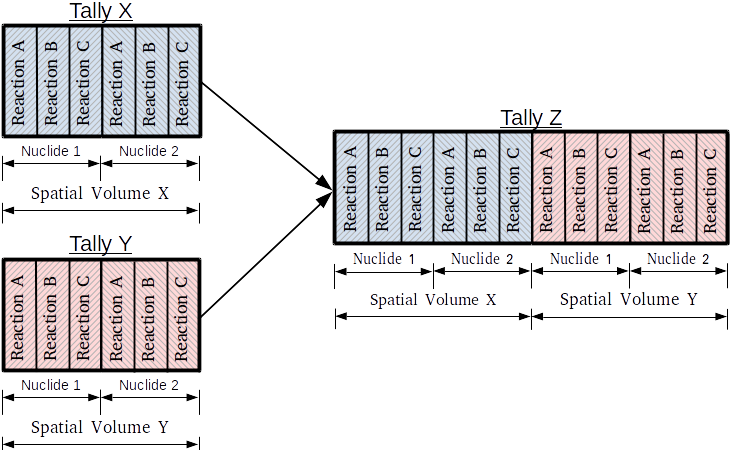
\includegraphics[width=0.6\linewidth]{figures/tally-merge}
  \caption{}
\end{subfigure}
\begin{subfigure}{\textwidth}
  \centering
  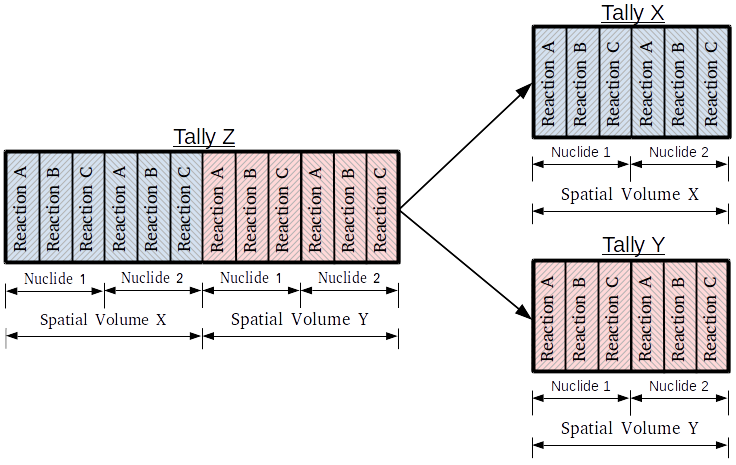
\includegraphics[width=0.6\linewidth]{figures/tally-slice}
  \caption{}
\end{subfigure}
\caption{Two \texttt{Tally} objects for different spatial volumes are merged into a single \texttt{Tally} (a). A single \texttt{Tally} is sliced by spatial volume into two distinct \texttt{Tally} objects (b).}
\label{fig:tally-merge-slice}
\end{figure}

%%%%%%%%%%%%%%%%%%%%%%%%%%%%%%%%
\subsubsection{Tally Arithmetic}
\label{subsubsec:tally-arithmetic}

A variety of reaction rate and flux tallies must be arithmetically combined in order to compute MGXS with Monte Carlo. At the most general level, a reaction rate tally must be divided by a flux tally for each energy group, nuclide and tally volume. The Python API provides a novel feature known as \textit{tally arithmetic} to enable arithmetic combinations of tallies with efficient vectorized numerical operations across energy groups, nuclides and spatial tally zones.

Tally arithmetic is an object-oriented data processing feature which arithmetically combines two or more tallies and/or scalar values into new \textit{derived tallies}. The tally arithmetic implementation in OpenMC overloads the operators for addition, subtraction, multiplication, division, and exponentiation in the Python API's \texttt{Tally} class. In addition, the \texttt{Tally} class supports summation or averaging operations across some or all of its filter, nuclide or score bins. The derived tallies produced from tally arithmetic provide the same rich functionality available for the \texttt{Tally} operands used in the arithmetic operation (\textit{e.g.}, Pandas DataFrames, tally arithmetic).

Multi-group cross sections may be simply and efficiently computed with tally arithmetic. For example, the following code snippet illustrates how tally slicing and arithmetic are used to compute a total MGXS. The total MGXS that is returned from the tally division operation is encapsulated within a \texttt{Tally} class. This is the approach used by the MGXS generation module created for OpenMC.

\lstinputlisting[language=Python, basicstyle=\ttfamily\scriptsize, caption={MGXS calculation with tally arithmetic.}, label={lst:python-input}]{listings/tally-arithmetic.py}

A primary objective of tally arithmetic is to rapidly transform tally data with automated uncertainty propagation. Estimates of the variance for derived tallies from tally arithmetic are deduced from standard error propagation theory~\cite{bevington2003data}. The division arithmetic operator is primarily used to to compute MGXS from MC tallies. Consider two random variables $X$ and $Y$, generated from distributions with variances $\sigma_{X}^2$ and $\sigma_{Y}^2$ which are divided into a new random variable $Z$ with variance $\sigma_{Z}^2$:

\begin{equation}
\label{eqn:div-prop}
\sigma_{Z}^{2} \approx Z^{2}\left[\left(\frac{\sigma_{X}}{X}\right)^{2} + \left(\frac{\sigma_{Y}}{Y}\right)^{2} - 2\frac{\sigma_{XY}}{Z}\right]
\end{equation}

\noindent The variables $X$ and $Y$ may correspond to tallies for reaction rates and the flux, while $Z$ could correspond to a MGXS.

The covariance $\sigma_{XY}$ is not generally computable using the standard formulation for a tally estimator in a Monte Carlo simulation. Although it would be possible to estimate the covariance using ensemble statistics, this is not often feasible. Instead, the covariance term in \cref{eqn:div-prop} is neglected by the current implementation of tally arithmetic. In general, the random variables for reaction rates and fluxes in the same volume of phase space are highly correlated, such that a conservative estimate of the variance for MGXS is obtained by neglecting the covariance.

%%%%%%%%%%%%%%%%%%%%%%%%%%%%%%%%%%%%%
\subsubsection{Distributed Cell Tallies}
\label{subsec:distribcells}

%Many Monte Carlo codes, including OpenMC, use some variant of combinatorial geometry (CG) because it can represent arbitrary, repeating geometries such as fuel pins and assemblies. However, the CG approach is challenged by applications which require tallies in each instance of a repeated cell throughout a reactor geometry. The ``brute force'' solution is to instantiate a unique cell for each distinct tally zone. However, this defeats the purpose of using CG for its compact representation, and it is not scalable to problems with large tally datasets such as those considered in this thesis.

The \textit{distributed cell tally} algorithm was implemented in OpenMC \cite{lax2014distribcell} to permit simply defined spatial tally zones across repeated cell instances. The distributed cell algorithm -- abbreviated as the \textit{distribcell} algorithm -- classifies each unique cell instance using a process which consumes orders of magnitude less memory than would be required by the ``brute force'' approach. Only a single transparent line of XML input is necessary to define a distribcell tally which may span across an arbitrary number of instances for a particular cell. Furthermore, the Python API may be used to perform efficient vectorized transformations of distribcell tally data stored as contiguous NumPy arrays. In particular, the distribcell tally algorithm may be used to compute spatially-varying MGXS across fuel pin cell instances.

%%%%%%%%%%%%%%%%%%%%%%%%%%%%%
\subsubsection{Multi-Group Mode}
\label{subsec:openmc-mg-mode}

\begin{itemize}[noitemsep]
\item support stochastic multi-group calculations
\item multiple scattering representations (Legendre moments, discrete bins)
\item use OpenMC to generate MGXS, then insert into identical model for MG calculation
\item mention angular-dependent MGXS, or save for later paper?
\end{itemize}

%%%%%%%%%%%%%%%%%%%%%%%%%%%%%%%%%%%%%%%%%%%%%%%%%%%%%%%%%%%%%%%%%%%%%%%%%%%%%%%
\subsection{Software Design}
\label{sec:software}
%%%%%%%%%%%%%%%%%%%%%%%%%%%%%%%%%%%%%%%%%%%%%%%%%%%%%%%%%%%%%%%%%%%%%%%%%%%%%%%

The OpenMC Python API's \texttt{openmc.mgxs} module was designed to generate multi-group cross sections. The \texttt{openmc.mgxs} module is built atop the underlying core features in the rest of the API to support a seamless interface for both input generation and downstream data processing of MGXS from Python. In particular, one may specify the MGXS to compute and the \texttt{openmc.mgxs} module will construct the necessary \texttt{Tally} objects. The \texttt{Tally} objects may be easily exported to XML input files for OpenMC, and used to containerize and process the tally data produced by an OpenMC simulation. The \texttt{openmc.mgxs} module thereby leverages the software stack (\textit{e.g.}, tally arithmetic, Pandas DataFrames) provided by the Python API.

The \texttt{openmc.mgxs} module uses an object-oriented design based on an abstract \texttt{MGXS} class with subclasses for different reaction types. The \texttt{MGXS} subclasses are itemized in \cref{tab:mgxs-types} and compute macroscopic or microscopic multi-group constants in one or more arbitrary energy group structures from MC tallies. The \texttt{openmc.mgxs} module also includes a \texttt{Library} class which automates the construction of \texttt{MGXS} objects for different group structures, spatial domains, and reaction types.

\begin{table}[h!]
  \centering
  \caption{The multi-group cross section types implemented by the \texttt{openmc.mgxs} module.}
  \small
  \label{tab:mgxs-types}
  \vspace{6pt}
  \begin{tabular}{l l}
  \toprule
  \textbf{Class} &
  \textbf{Description} \\
  \midrule
  \multicolumn{2}{c}{\bf Prompt Neutron Constants} \\
  \midrule
  \texttt{AbsorptionXS} & Absorption \\
  \texttt{CaptureXS} & Radiative capture \\
  \texttt{Chi} & Fission emission spectrum \\
  \texttt{FissionXS} & Fission \\
  \texttt{InverseVelocity} & Inverse neutron velocity \\
  \texttt{KappaFissionXS} & Fission energy release \\
  \texttt{MultiplicityMatrixXS} & Scattering multiplicity matrix \\
  \texttt{NuFissionMatrixXS} & Fission production matrix \\
  \texttt{ScatterXS} & Scattering \\
  \texttt{ScatterMatrixXS} & Scattering matrix \\
  \texttt{ScatterProbabilityMatrixXS} & Scattering probability matrix \\
  \texttt{TotalXS} & Total collision \\
  \texttt{TransportXS} & Transport-corrected total collision \\
  \midrule
  \multicolumn{2}{c}{\bf Delayed Neutron Constants} \\
  \midrule
  \texttt{Beta} & Delayed neutron fraction \\
  \texttt{ChiDelayed} & Delayed fission spectrum \\
  \texttt{DecayRate} & Delayed neutron precursors decay rate \\
  \texttt{DelayedNuFissionXS} & Fission delayed neutron production \\
  \texttt{DelayedNuFissionMatrixXS} & Fission delayed neutron production matrix \\
  \bottomrule
\end{tabular}
\end{table}


%%%%%%%%%%%%%%%%%%%%%%%%%%%%%
\subsubsection{XML Input Generation}
\label{subsec:xml-inputs}

\begin{itemize}[noitemsep]
\item workflow: create Python model, create \texttt{Library}, export to XML
\item code snippet?
\end{itemize}

%%%%%%%%%%%%%%%%%%%%%%%%%%%%%
\subsubsection{Data Processing}
\label{subsec:data-processing}

\begin{itemize}[noitemsep]
\item refer to PyAPI features that are ``inherited'' by \texttt{openmc.mgxs}:
  \begin{itemize}[noitemsep]
  \item Pandas DataFrames, tally arithmetic/slicing/merging, ...
  \end{itemize}
\end{itemize}

%%%%%%%%%%%%%%%%%%%%%%%%%
\subsubsection{Data Storage}
\label{subsec:data-storage}

The \texttt{openmc.mgxs} module was developed with general design principles to generate MGXS for any multi-group neutron transport code. Although the module does not explicitly support any multi-group codes, it can export MGXS data to a variety of data storage formats, including Comma-Separated Values (CSV) and HDF5. The exported MGXS files may be easily transformed into the database or input files required by a particular multi-group code.

%%%%%%%%%%%%%%%%%%%%%%%%%%%%%%%%%%%%%%%%%%%%%%%%%%%%%%%%%%%%%%%%%%%%%%%%%%%%%%%
\subsection{Features}
\label{sec:features}
%%%%%%%%%%%%%%%%%%%%%%%%%%%%%%%%%%%%%%%%%%%%%%%%%%%%%%%%%%%%%%%%%%%%%%%%%%%%%%%


%%%%%%%%%%%%%%%%%%%%%%%%%%%%%%%%%%%%%%%%%%%%
\subsubsection{Energy Condensation}
\label{subsec:energy-condense}

The module supports energy condensation in downstream data processing which is useful for exploring approximation bias in various energy group structures. For example, MGXS may be computed in some ``fine'' energy group structure and the tally data subsequently condensed to some coarser group structure \texttt{coarse_groups} for multi-group calculations with the \texttt{MGXS.get_condensed_xs(coarse_groups)} Python class method. Energy condensation may be performed to arbitrarily defined coarse group structures provided the coarse group boundaries coincide with boundaries in the fine group structure.


%%%%%%%%%%%%%%%%%%%%%%%%%%%%%%%%%%%%%%%%%%%%
\subsubsection{Pin-Wise Spatial Homogenization}
\label{subsec:pinwise-homogenize}

The \texttt{openmc.mgxs} module is designed to perform spatial homogenization on heterogeneous tally meshes for fine-mesh transport codes. In OpenMC parlance, MGXS may be computed for material, cell or universe spatial domains. In addition, the module supports MGXS calculations for repeated cell instances using distribcell spatial tally domains\cite{lax2014distribcell}. Spatial homogenization across some subset of distributed cell instances \texttt{cell_instances} can be performed using the \texttt{MGXS.get_subdomain_avg_xs(cell_instances)} Python class method.

%The \texttt{openmc.mgxs} module may also perform spatial homogenization on structured Cartesian tally meshes for coarse mesh multi-group calculations..


%%%%%%%%%%%%%%%%%%%%%%%%%%%%%%%%%%%%%%%%%%%%
\subsubsection{Microscopic MGXS}
\label{subsec:micro-macro}

I hear it is unique that we can calculate micros?


%%%%%%%%%%%%%%%%%%%%%%%%%%%%%%%%%%%%%%%%
\subsubsection{Isotropic in Lab Scattering}
\label{subsec:iso-in-lab}

A unique option for isotropic in lab scattering is implemented in the OpenMC code. The isotropic in lab feature, abbreviated as \textit{iso-in-lab}, may be useful to quantify the ability of multi-group codes to capture anisotropic scattering effects with higher order scattering matrices or transport correction schemes. The iso-in-lab feature is implemented as an optional attribute for each nuclide or element in a simulation. When iso-in-lab scattering is specified for a nuclide or element, the outgoing neutron energy is sampled from the scattering laws prescribed by the continuous energy cross section library, but the outgoing neutron direction of motion is sampled from an isotropic in lab distribution.

%%%%%%%%%%%%%%%%%%%%%%%%%%%%%
\subsection{Tally Estimators}
\label{subsec:tally-est}

\begin{itemize}[noitemsep]
\item Table of the tally estimators acceptable for each MGXS type
\item Mention tally estimators can be toggled? Or discuss in software design?
\item Add footnote mentioning consistent scattering formulation
\end{itemize}

\begin{table}[h!]
  \centering
  \caption{The tally estimators supported by each MGXS type.}
  \small
  \label{tab:mgxs-tally-estimators}
  \vspace{6pt}
  \begin{tabular}{l c c c}
  \toprule
  \textbf{Class} &
  \textbf{Analog} &
  \textbf{Collision} &
  \textbf{Track-length} \\
  \midrule
  \multicolumn{4}{c}{\bf Prompt Neutron Constants} \\
  \midrule
  \texttt{AbsorptionXS} & \cmark & \cmark & \cmark \\
  \texttt{CaptureXS} & \cmark & \cmark & \cmark \\
  \texttt{Chi} & \cmark & \xmark & \xmark \\
  \texttt{FissionXS} & \cmark & \cmark & \cmark \\
  \texttt{InverseVelocity} & \cmark & \cmark & \cmark \\
  \texttt{KappaFissionXS} & \cmark & \cmark & \cmark \\
  \texttt{MultiplicityMatrixXS} & \cmark & \xmark & \xmark \\
  \texttt{NuFissionMatrixXS} & \cmark & \xmark & \xmark \\
  \texttt{ScatterXS} & \cmark & \cmark & \cmark \\
  \texttt{ScatterMatrixXS} & \cmark & \xmark & \xmark \\
  \texttt{ScatterProbabilityMatrixXS} & \cmark & \xmark & \xmark \\
  \texttt{TotalXS} & \cmark & \cmark & \cmark \\
  \texttt{TransportXS} & \cmark & \xmark & \xmark \\
  \midrule
  \multicolumn{4}{c}{\bf Delayed Neutron Constants} \\
  \midrule
  \texttt{Beta} & \cmark & \cmark & \cmark \\
  \texttt{ChiDelayed} & \cmark & \xmark & \xmark \\
  \texttt{DecayRate} & \cmark & \cmark & \cmark \\
  \texttt{DelayedNuFissionXS} & \cmark & \cmark & \cmark \\
  \texttt{DelayedNuFissionMatrixXS} & \cmark & \xmark & \xmark \\
  \bottomrule
\end{tabular}
\end{table}
